\def\assignmenttitle{Assignment 2}
\def\assignmentdate{08-12-2011}
\def\assignmentnumber{2}

\documentclass[11pt]{article}
\linespread{1}

\renewcommand{\thefootnote}{\fnsymbol{footnote}}

\usepackage{geometry} % see geometry.pdf on how to lay out the page. There's lots.
\usepackage[utf8]{inputenc}
\usepackage[T1]{fontenc}
\usepackage{array}
\usepackage{amsmath,amssymb,latexsym,epic,eepic,epsfig,graphics,psfrag}
\usepackage{amsfonts}
\usepackage{graphicx,float}
\usepackage{color}
\definecolor{mygray}{RGB}{244,244,244}
\definecolor{gray}{gray}{0.5}
\definecolor{myredish}{RGB}{193,33,97}
\definecolor{grayblue}{RGB}{91,112,142}
\definecolor{myorange}{RGB}{255,134,0}
\definecolor{green}{rgb}{0,0.4,0}

\usepackage[english]{babel}

\usepackage[bottom]{footmisc}

\usepackage{fancyhdr}
\pagestyle{fancy}
\lhead{\small\textit{Assignment \assignmentnumber -- 02417 Time Series Analysis -- Anders Hørsted (s082382)}}
\rhead{\thepage}
\chead{}
\lfoot{}\cfoot{}\rfoot{}

\usepackage{subfigure}
\usepackage{pstricks}
\usepackage{pst-node}
\usepackage{wrapfig}
\usepackage{caption}
\usepackage{multirow}
%\usepackage{fouriernc}
%\usepackage[charter]{mathdesign}
\usepackage{lmodern}
\usepackage[normalem]{ulem}
\geometry{a4paper} % or letter or a5paper or ... etc
% \geometry{landscape} % rotated page geometry

\usepackage{url}


\makeatletter
\renewcommand*\env@matrix[1][*\c@MaxMatrixCols c]{%
  \hskip -\arraycolsep
  \let\@ifnextchar\new@ifnextchar
  \array{#1}}
\makeatother

\newcommand\myimp{\quad\Leftrightarrow\quad}
\newcommand\half{\frac{1}{2}}
\newcommand\myvec[1]{\mathbf{#1}}
\newcommand\mymod[1]{\ (\text{mod }#1)}
\newcommand\myreal{\mathbb{R}}
\newcommand\mynatural{\mathbb{N}}
\newcommand\myinteger{\mathbb{Z}}
\newcommand\mycomplex{\mathbb{C}}
\newcommand\myint{\text{int}}
\newcommand\norm[1]{||\,#1\,||}
\newcommand\bignorm[1]{\big|\big|\,#1\,\big|\big|}
\newcommand\seq[1]{\big\{#1\big\}}
\newcommand\smallseq[1]{\{#1\}}
\newcommand\smallseqtoinf[1]{\smallseq{#1}_{k=1}^\infty}
\newcommand\lonew{\ell^1_w}
\newcommand\lone{\ell^1}
\newcommand\ltwo{\ell^2(\mynatural)}
\newcommand\ip[2]{\langle#1,#2\rangle}
\newcommand\hilbert[1]{\mathcal{#1}}
\newcommand\uinf{u_{\infty}}
\newcommand\erf{\text{erf\,}}
\newcommand\infint{\int_{\infty}^{\infty}}
\newcommand\fpi{FPI}
\newcommand\E[1]{\text{E}[#1]}
\newcommand\Var[1]{\text{Var}[#1]}
\newcommand\Cov[1]{\text{Cov}[#1]}
\newcommand\myverb[1]{{\footnotesize\texttt{#1}}}
\newcommand\Yhat{\widehat{Y}}
\newcommand\given{\,|\,}

\usepackage[scaled]{beramono}
\usepackage{listings}
\lstset {                 % A rudimentary config that shows off some features.
    language=R,
    basicstyle=\scriptsize\ttfamily, % Without beramono, we'd get cmtt, the teletype font.
    commentstyle=\textit, % cmtt doesn't do italics. It might do slanted text though.
    keywordstyle=,
    identifierstyle=,
    framextopmargin=4pt,
    framexbottommargin=4pt,
    framexleftmargin=4pt,
    framexrightmargin=4pt,
    xleftmargin=4pt,
    xrightmargin=4pt,
    backgroundcolor=\color{mygray},
    frame=single,
    showstringspaces=false,
    captionpos=b,
    tabsize=4            % Or whatever you use in your editor, I suppose.
}

\renewcommand{\lstlistlistingname}{Code Listings}
\renewcommand{\lstlistingname}{Code Listing}

\usepackage{tabulary}
\newcolumntype{y}{>{\centering\arraybackslash}R}

\title{\assignmenttitle}
\date{\assignmentdate}
\author{Assignment \assignmentnumber\ -- 02417 Time Series Analysis -- Anders Hørsted (s082382)}
%\author{}
\date{} % delete this line to display the current date



\begin{document}

\maketitle


\section*{Question 1: Fitting to Air Pollution Data}

In this question we are going to fit sums of sines and cosines to the Air
Pollution Data given in the assignment. First a function \myverb{NOfit} that
calculates the parameters and the residuals for the fit is created.

\subsection*{Question 1.1}

The function should have the call \myverb{[x\_star, r\_star] = NOfit(t,y,n)},
but for convenience it is written to also return the design matrix $A$. The
function \myverb{NOfit} relies on \myverb{get\_A} to calculate the actual
design matrix. The function \myverb{get\_A} is used later when the fits are
plotted.

\lstinputlisting[caption={\myverb{NOfit} function to fit sine, cosines of order \myverb{n}}]{../src/NOfit.m}

\lstinputlisting[caption={Helper function \myverb{get\_A} used to generate design matrix}]{../src/get_A.m}

\subsection*{Question 1.2}

\coderemark{ex12} 

The \myverb{NOfit} function is now tested. Using the data given in the
assignment text a 3rd order cosine is fitted which gives the model. 

\begin{equation*}
    M(\myvec{x}, t) = 186.81 -44.94 \sin(\omega t) -93.43 \cos(\omega t)
\end{equation*}

To confirm the implementation of \myverb{NOfit} the residual 2-norm is checked
and it is the expected $\norm{\myvec{r^*}}_2=292.558$. Since the implementation
seems to be right, the fitted model is plotted along with the data in
figure~\ref{fig:3rd-order-fit} .\par

\begin{figure}[ht]
    \centering
    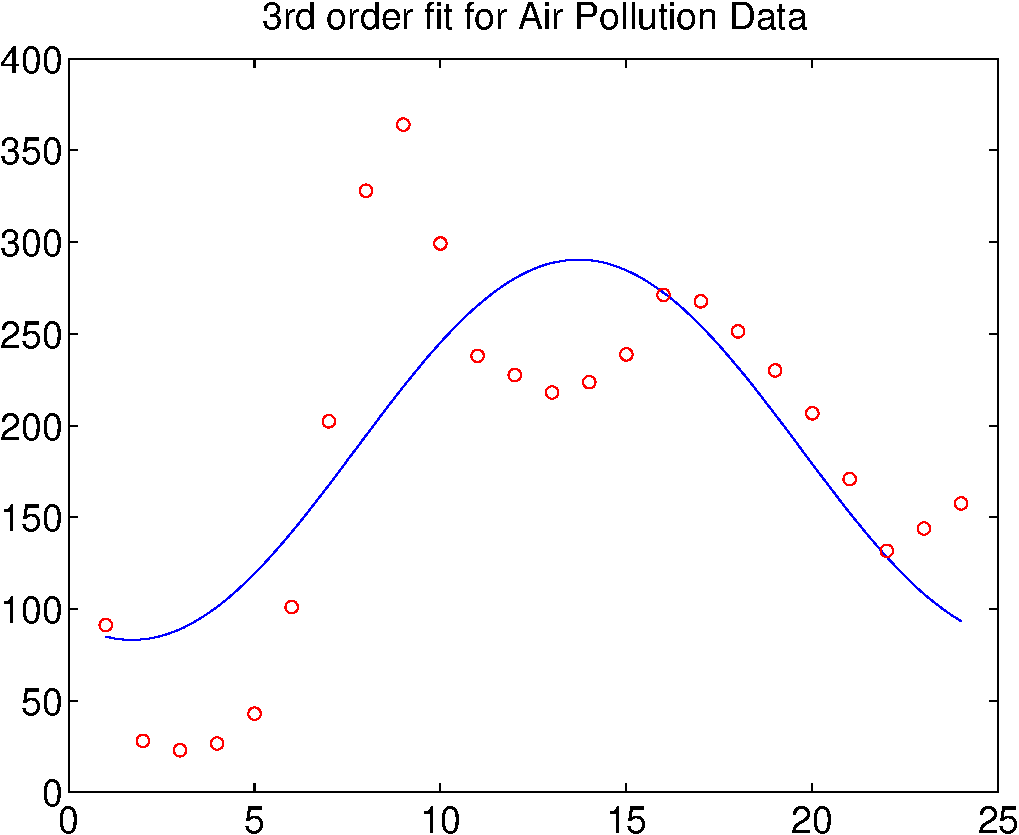
\includegraphics[width=70mm]{../media/3rd-order-fit.pdf}
    \caption{CAPTION!!!}
    \label{fig:3rd-order-fit}
\end{figure}

\subsection*{Question 1.3}

\coderemark{ex13}

The optimal order of the fit must be determined. Using the test for random
signs and the test for correlation, for the orders $n=3,5,7,9,11,13$ gives the
results shown in figure~\ref{fig:ex13}.

\begin{figure}
    \centering
    \mbox{  \subfigure{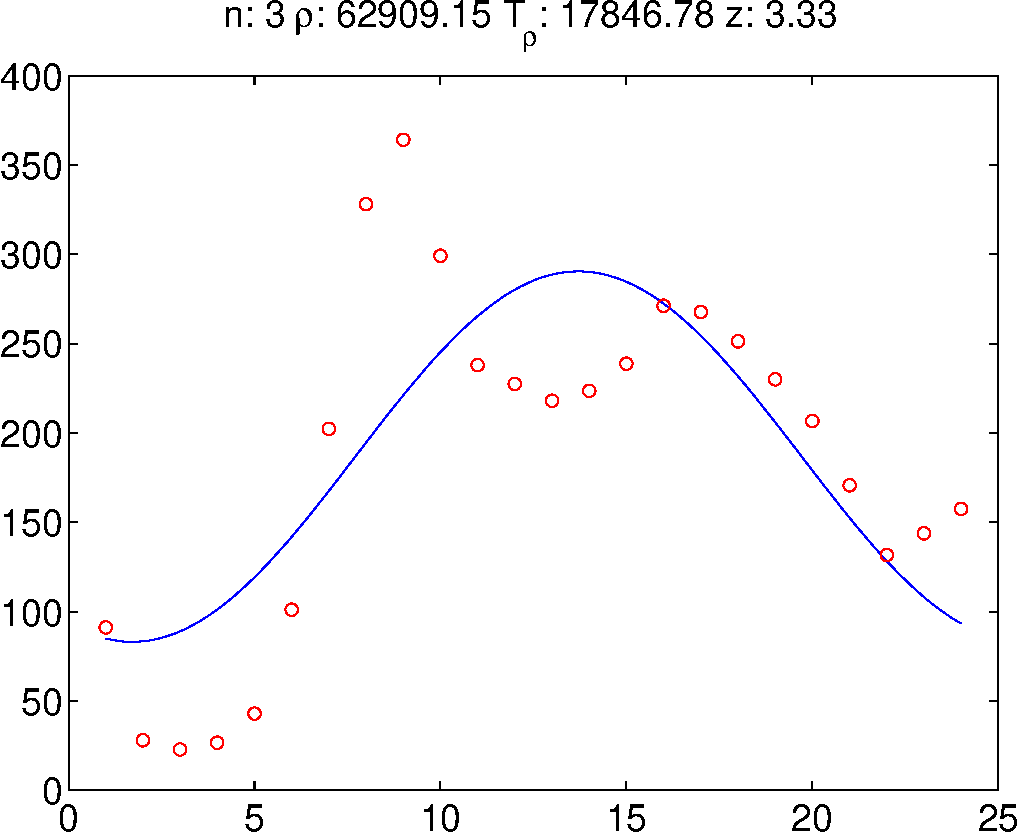
\includegraphics[width=70mm]{../media/order-determination-3.pdf}} \quad 
            \subfigure{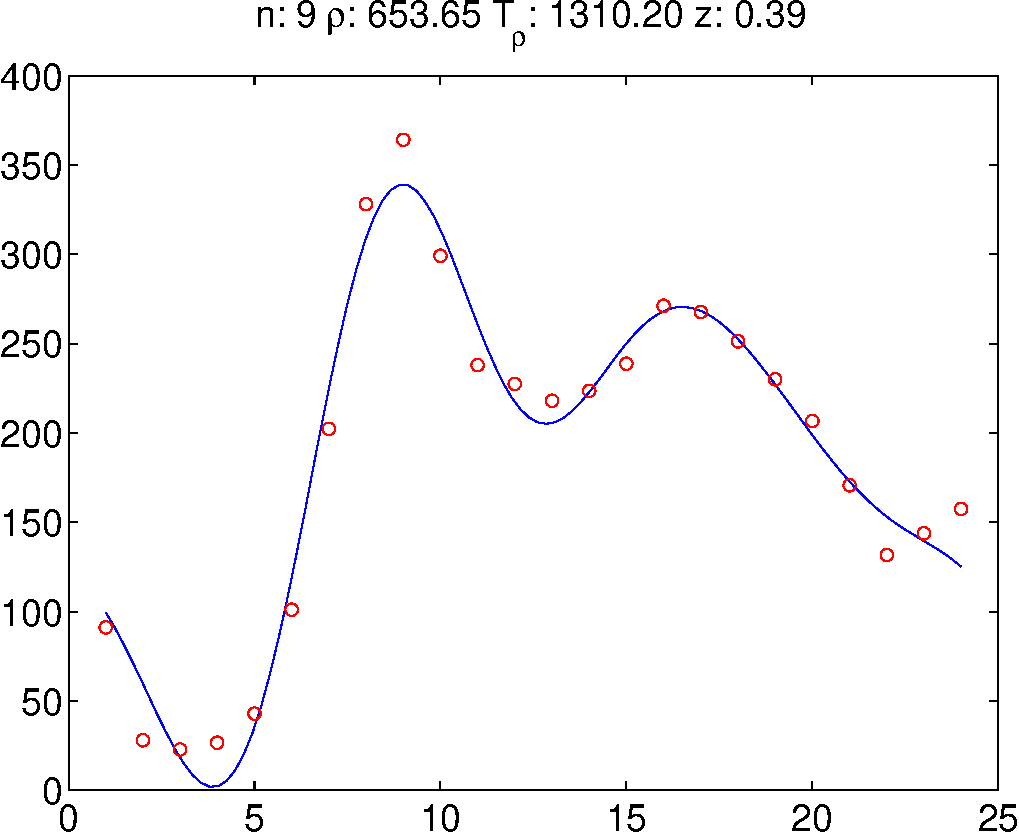
\includegraphics[width=70mm]{../media/order-determination-9.pdf}}}
    \mbox{\vspace{5mm}}
    \mbox{  \subfigure{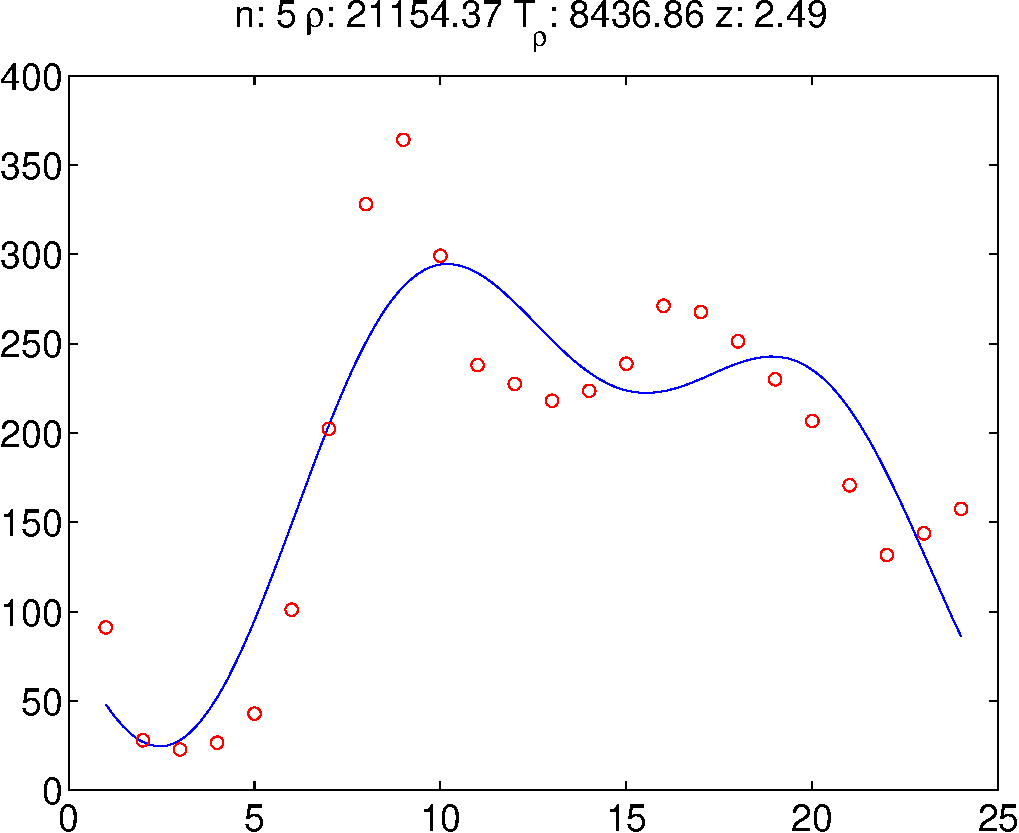
\includegraphics[width=70mm]{../media/order-determination-5.pdf}} \quad 
            \subfigure{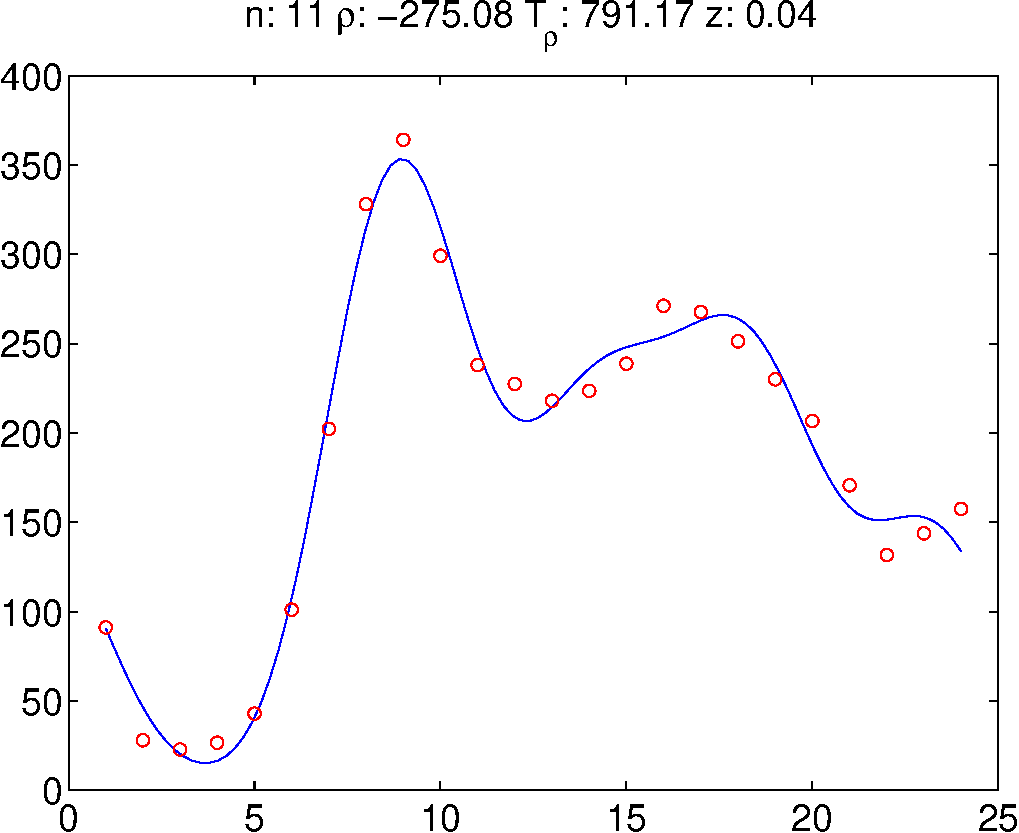
\includegraphics[width=70mm]{../media/order-determination-11.pdf}}}
    \mbox{\vspace{5mm}}
    \mbox{  \subfigure{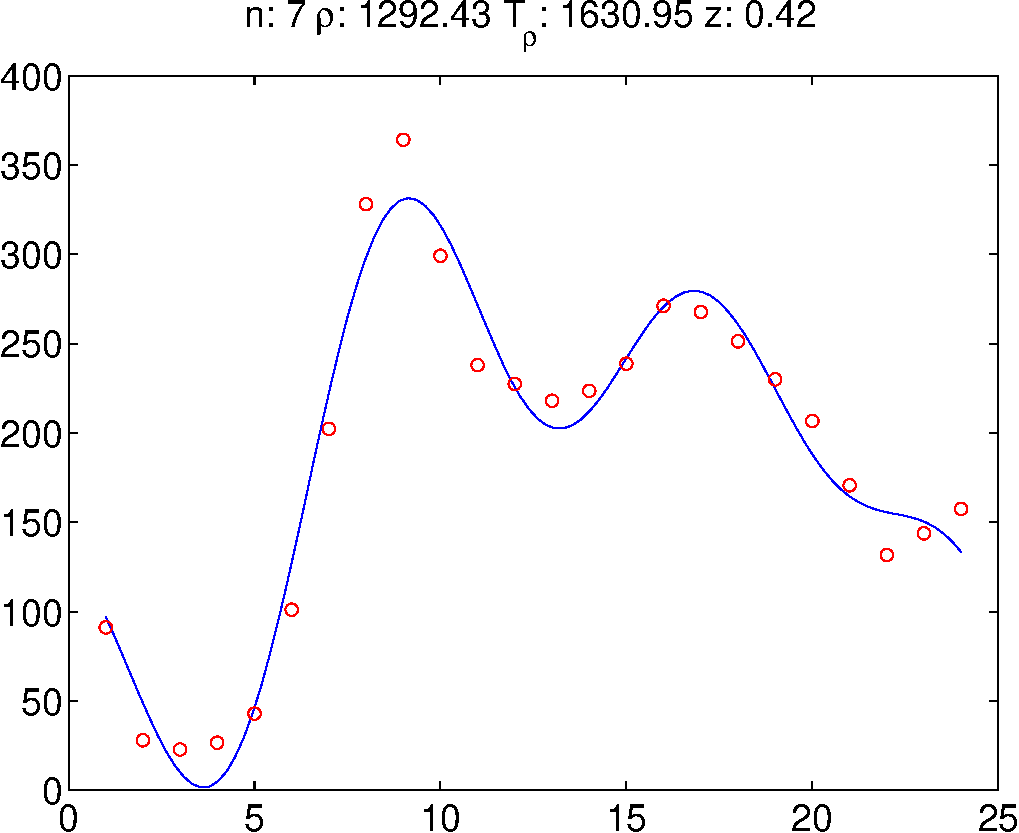
\includegraphics[width=70mm]{../media/order-determination-7.pdf}} \quad 
            \subfigure{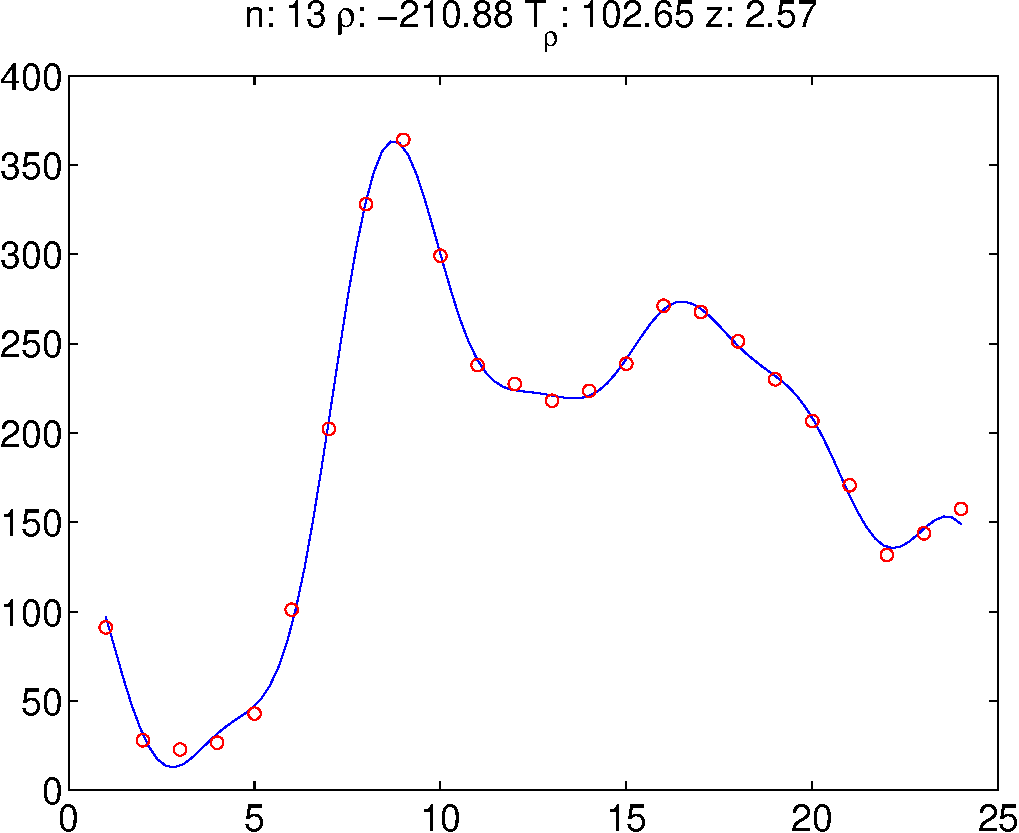
\includegraphics[width=70mm]{../media/order-determination-13.pdf}}}
    \caption{CAPTION!!!}
    \label{fig:ex13}
\end{figure}

\pagebreak
\renewcommand\thesection{\Alph{section}}


\section{Appendices}

All \matlab\ source code is included in the appendices. All the source code
including the LaTex code used for the report can also be found at
\url{https://github.com/alphabits/dtu-fall-2011/tree/master/02610/assignment-2}.

\subsection{Question 1.2}\label{app:ex12}
\lstinputlisting[caption={ex12.m}]{../src/ex12.m}

\subsection{Question 1.3}\label{app:ex13}
\lstinputlisting[caption={ex13.m}]{../src/ex13.m}

\subsection{Helper functions}\label{app:helpers}
\lstinputlisting[caption={plot\_fit.m}]{../src/plot_fit.m}
\lstinputlisting[caption={plot\_fit\_with\_res\_analysis.m}]{../src/plot_fit_with_res_analysis.m}

\pagebreak
\begin{thebibliography}{9}

\bibitem{hm}
  Henrik Madsen,
  \emph{Time Series Analysis}.
  Chapman \& Hall/CRC,
  1st Edition,
  2008.

%\bibitem{taleb}
%  Nassim Nicholas Taleb,
%  \emph{The Black Swan}.
%  Random House Trade Paperbacks
%  2nd Edition,
%  2010.

\end{thebibliography}


\end{document}
